\chapter{Dyons on \texorpdfstring{$\KT$}{K3 x T2}: From the Elliptic Genus to Class Numbers}\label{ch:dyons}

A black hole carries electric and magnetic charge. If string theory is a quantum theory of
gravity, it must say how many quantum states hide behind those charges --- not approximately,
but as an integer, for every allowed charge vector. For type II string theory on $\KT$ that
integer is known in closed form, and the closed form is a Fourier coefficient of one
meromorphic function of three variables. This chapter answers the question: \emph{where does
that function come from, what makes it meromorphic rather than holomorphic, and what survives
when the poles are removed?} The answer to the last part is the small surprise of the chapter:
what survives at the simplest charge is a generating function of \emph{class numbers} of
imaginary quadratic forms, objects a student meets in a first course on number theory and
would never expect to meet again in a black-hole count.

Along the way the student learns three techniques that recur throughout this book: building a
modular object as an infinite product whose exponents are the Fourier coefficients of a
simpler object (\cref{sec:dyons:product}); separating a meromorphic function into a polar part
fixed entirely by its poles and a remainder (\cref{sec:dyons:polar}); and testing an integer
coincidence by replacing dimensions with characters (\cref{sec:dyons:twining}). Everything in
\cref{sec:dyons:lean} is exact integer arithmetic that the Lean kernel re-checks.

Conventions. As in \cref{ch:ellgenus}, $q=\ee^{2\pi\ii\tau}$, $y=\ee^{2\pi\ii z}$, and
$p=\ee^{2\pi\ii\sigma}$; $\eta$ is the Dedekind eta function, $\Delta=\eta^{24}$, and
$E_4,E_6$ are the Eisenstein series of weight $4$ and $6$. The elliptic genus of K3 is
$Z(\tau,z)=2\phi_{0,1}(\tau,z)$, twice the standard weak Jacobi form of weight $0$ and index
$1$; $A:=\phi_{-2,1}$ and $B:=\phi_{0,1}$ throughout, following
Dabholkar--Murthy--Zagier \source{DMZ §9.1, ll.~3629--3634}.

\section{Dyons, their charges, and what we are counting}\label{sec:dyons:charges}

Compactifying type II string theory on $\KT$ gives a four-dimensional theory with $N=4$
supersymmetry \source{Asp §7, ll.~2741--2745}. A state is labelled by an electric charge
vector $N$ and a magnetic charge vector $M$, both living in the even self-dual lattice
$\Pi^{22,6}$; a state is \emph{dyonic}\index{dyon} when both are non-zero
\source{DMZ §2.2, ll.~638--645}. The duality group does not see $N$ and $M$ separately: the
three T-duality invariants\index{T-duality!invariants} are
\begin{equation}\label{eq:dyons:invariants}
  (m,n,\ell)\;=\;\Bigl(\tfrac{M^2}{2},\ \tfrac{N^2}{2},\ N\cdot M\Bigr),
\end{equation}
all integers because $\Pi^{22,6}$ is integral \source{DMZ §2.3, ll.~744--748}. The counting
problem splits in two.

\emph{Half-BPS states} preserve half the supersymmetry. Their degeneracy depends on $n$ only,
and is
\begin{equation}\label{eq:dyons:halfbps}
  d(n)=p_{24}(n+1),\qquad \frac{1}{\Delta(\tau)}=\sum_{n\ge-1}p_{24}(n+1)\,q^{n},
\end{equation}
where $p_{24}(I)$\index{colored partitions}\index{p24@$p_{24}$} counts partitions of $I$ into
parts of $24$ colours \source{DMZ §3.4, ll.~1066--1071}. The $24$ is the number of transverse
oscillators of the heterotic string --- and, on the type II side, the Euler number of K3. These
states never decay: the degeneracy is the same everywhere in moduli space.

\emph{Quarter-BPS states} are the interesting ones. Their degeneracy \emph{does} depend on
where one sits in moduli space: a bound state of two half-BPS constituents exists in one
region and does not exist in another, and the count jumps across a \emph{wall of marginal
stability}\index{wall of marginal stability} \source{DMZ §6, ll.~1997--2004}. All of them are
packaged in one generating function,
\begin{equation}\label{eq:dyons:Z}
  \frac{1}{\Phi_{10}(\Omega)}=\sum_{m\ge-1}\psi_m(\tau,z)\,p^{m},
  \qquad
  \Omega=\begin{pmatrix}\tau&z\\ z&\sigma\end{pmatrix},
\end{equation}
the reciprocal of the Igusa cusp form of weight $10$ \source{DMZ §1.1, ll.~172--183}. The
degeneracy $d(m,n,\ell)$ is a Fourier coefficient of \eqref{eq:dyons:Z} along a contour whose
choice encodes the moduli \source{DMZ §6, ll.~1982--1990}. Everything in this chapter concerns
the functions $\psi_m$, one for each magnetic charge invariant $m$.

\begin{physicsbox}[Why a pole is a physical statement]
A holomorphic generating function would give one degeneracy per charge, full stop. The
function \eqref{eq:dyons:Z} has \emph{poles}, and the Fourier coefficient therefore depends on
which side of a pole the integration contour runs. That is exactly the physics of wall
crossing: two-centred configurations appear or disappear, and the count jumps by the residue
\source{DMZ §6, ll.~2000--2006}. A pole in a partition function is not a defect; it is where
the decay of bound states is recorded.
\end{physicsbox}

\section{Two Jacobi forms, and the elliptic genus}\label{sec:dyons:AB}

Every weak Jacobi form of index $1$ is a modular-form combination of two generators, of weight
$-2$ and $0$. In terms of theta functions \source{DMZ §4.3, ll.~1416--1424},
\begin{equation}\label{eq:dyons:ABtheta}
  A=\phi_{-2,1}=\frac{\vartheta_1(\tau,z)^2}{\eta(\tau)^6},
  \qquad
  B=\phi_{0,1}=4\left(\frac{\vartheta_2(\tau,z)^2}{\vartheta_2(\tau)^2}
   +\frac{\vartheta_3(\tau,z)^2}{\vartheta_3(\tau)^2}
   +\frac{\vartheta_4(\tau,z)^2}{\vartheta_4(\tau)^2}\right),
\end{equation}
with the expansions \source{DMZ §4.3, ll.~1397--1402}
\begin{equation}\label{eq:dyons:ABq}
  A=\frac{(y-1)^2}{y}-2\frac{(y-1)^4}{y^2}q+\cdots,
  \qquad
  B=\frac{y^2+10y+1}{y}+2\frac{(y-1)^2(5y^2-22y+5)}{y^2}q+\cdots .
\end{equation}
Two features of \eqref{eq:dyons:ABq} will be used constantly: as $z\to0$,
\begin{equation}\label{eq:dyons:ABlimits}
  A(\tau,z)\sim(2\pi\ii z)^2\longrightarrow 0,
  \qquad
  B(\tau,z)\longrightarrow 12 ,
\end{equation}
\source{DMZ §9.1, ll.~3633--3635}. The K3 elliptic genus is $Z=2B$, and since coefficients of
an index-$1$ form depend only on the discriminant $\Delta=4n-l^2$ we may write
$Z=\sum c(4n-l^2)q^ny^l$ with $c=2C_0$. The first values, read off Table~1 of DMZ
\source{DMZ §4.3, ll.~1404--1408}, are
\begin{equation}\label{eq:dyons:cvalues}
  c(-1)=2,\quad c(0)=20,\quad c(3)=-128,\quad c(4)=216,
\end{equation}
and $Z(\tau,0)=24=\chi(\mathrm{K3})$ \source{DMZ §4.5, ll.~1675--1681}.

\section{The partition function as a product}\label{sec:dyons:product}

The bridge from K3 to black holes is a product formula. Let $\chi(\tau,z;\mathrm{Sym}^k\mathrm{K3})$
be the elliptic genus of the $k$-th symmetric product of K3 and set
$\widehat Z=\sum_k\chi(\tau,z;\mathrm{Sym}^{k}\mathrm{K3})\,p^{k-1}$. Then
\source{DMZ §4.5, ll.~1688--1698}
\begin{equation}\label{eq:dyons:dmvv}
  \sum_{k\ge0}G_k(\tau,z)\,p^{k}
  \;=\;\prod_{\substack{r\ge1,\ s\ge0,\ t\in\Z}}\bigl(1-p^{r}q^{s}y^{t}\bigr)^{-c(4rs-t^2)},
  \qquad G_k=\chi(\tau,z;\mathrm{Sym}^{k}\mathrm{K3}),
\end{equation}
and the Igusa form itself is the same product with the opposite sign in the exponent and one
extra factor \source{DMZ §5.1, ll.~1816--1827}. Combining \eqref{eq:dyons:Z} with
\eqref{eq:dyons:dmvv} gives the working formula of this chapter,
\begin{equation}\label{eq:dyons:psiG}
  \Delta(\tau)\,\psi_m(\tau,z)=\frac{G_{m+1}(\tau,z)}{A(\tau,z)} .
\end{equation}
Note what \eqref{eq:dyons:dmvv} does: the \emph{input} is the K3 elliptic genus, one weak
Jacobi form; the \emph{output} is the full dyon partition function. Nothing else enters.

\subsection*{Worked example: the coefficient of \texorpdfstring{$p^2$}{p2} at $z=0$}

Set $y=1$ in \eqref{eq:dyons:dmvv}. The exponent of the factor $(1-p^rq^s)$ becomes
$\sum_t c(4rs-t^2)$, which is the sum of all $y$-coefficients of $Z$ at order $q^{rs}$. Since
$Z(\tau,0)=24$ is a constant in $q$, that sum is $24$ for $rs=0$ and $0$ otherwise. Only the
$s=0$ factors survive:
\begin{equation}\label{eq:dyons:goettsche}
  \sum_k G_k(\tau,0)\,p^k=\prod_{r\ge1}(1-p^r)^{-24}
  \quad\Longrightarrow\quad G_k(\tau,0)=p_{24}(k).
\end{equation}
For $k=2$, expand by hand: $(1-p)^{-24}$ contributes $\binom{25}{2}=300$ at order $p^2$ and
$(1-p^2)^{-24}$ contributes $24$, so $G_2(\tau,0)=324$. The same argument gives
$1,24,324,3200,25650,176256$ for $k=0,\dots,5$ --- the Euler numbers of the Hilbert schemes of
points on K3, Göttsche's numbers\index{Göttsche numbers}, and the half-BPS degeneracies
\eqref{eq:dyons:halfbps} again. The $24$ of K3 propagates to every order.

\begin{pitfallbox}[A truncated product can silently lie]
To compute $G_k$ through order $q^Q$ from \eqref{eq:dyons:dmvv} one needs the coefficients
$c(D)$ for all $D=4rs-t^2$ with $r\le k$, $s\le Q$ --- that is, up to $D=4kQ$. If the table of
$c$ stops earlier, the missing exponents are silently taken as $0$ and the answer is wrong
while looking perfectly regular. In the formalization this is not left to care: the
discriminants the product actually reads are enumerated and checked against what the computed
$Z$ provides (\lean{dmvv\_reachable}), together with a deliberately too-deep truncation that
fails the same test (\lean{dmvv\_unreachable\_example}).
\end{pitfallbox}

\subsection*{An independent check: the additive formulas}

The same $\psi_m$ can be written as polynomials in $A,B,E_4,E_6$ divided by $A$
\source{DMZ §5.2, ll.~1878--1888}:
\begin{align}\label{eq:dyons:516}
  \Delta\psi_{-1}&=A^{-1}, &
  \Delta\psi_{0}&=2A^{-1}B, \notag\\
  4\Delta\psi_{1}&=9A^{-1}B^2+3E_4A, &
  27\Delta\psi_{2}&=50A^{-1}B^3+48E_4AB+10E_6A^2 .
\end{align}
These are \emph{not} how we computed $G_k$; they are an independent route, and their agreement
with the product is a genuine test of both. A one-line consistency check at $z=0$ uses
\eqref{eq:dyons:ABlimits}: the third equation reads $4G_2=9B^2+3E_4A^2$, and at $z=0$ this is
$4\cdot324=9\cdot144=1296$. \Cref{sec:dyons:lean} records the full check through order $q^2$.

\section{The double pole and the two-centred states}\label{sec:dyons:polar}

By \eqref{eq:dyons:psiG} and \eqref{eq:dyons:ABlimits}, $\Delta\psi_m$ has a \emph{double} pole
at $z=0$, with principal part
\begin{equation}\label{eq:dyons:principal}
  \Delta(\tau)\psi_m(\tau,z)\;\sim\;\frac{p_{24}(m+1)}{(2\pi\ii z)^{2}} ,
\end{equation}
because the numerator tends to $G_{m+1}(\tau,0)=p_{24}(m+1)$ \source{DMZ §9.1, ll.~3622--3627}.
The pole is where the wall crossing lives, so one would like to subtract it in a canonical way.
Zwegers' theory, as recast by DMZ, does exactly this: there is a decomposition
\begin{equation}\label{eq:dyons:decomp}
  \psi_m=\psi^{P}_m+\psi^{F}_m,
  \qquad
  \psi^{P}_m=\frac{p_{24}(m+1)}{\Delta(\tau)}\,A_{2,m}(\tau,z),
\end{equation}
in which the \emph{polar part} $\psi^P_m$ is an elementary function determined by the poles
alone, and the \emph{finite part} $\psi^F_m$ has no poles at all
\source{DMZ §1.1, ll.~196--206}. Physically \source{DMZ §1.2, ll.~424--443}: $\psi^P_m$ counts
multi-centred (here: two-centred) configurations, whose number depends on the moduli;
$\psi^F_m$ counts \emph{single-centred}, or ``immortal'', black holes, whose count does not.
The elementary function is an Appell--Lerch sum\index{Appell--Lerch sum}
\source{DMZ §9.1, ll.~3658--3663}
\begin{equation}\label{eq:dyons:A2m}
  A_{2,m}(\tau,z)=\sum_{s\in\Z}\frac{q^{ms^2+s}\,y^{2ms+1}}{(1-q^sy)^2}.
\end{equation}

\begin{pitfallbox}[``The'' Fourier expansion of $A_{2,m}$ does not exist]
The summand of \eqref{eq:dyons:A2m} has poles at $y=q^{-s}$, so the Fourier expansion depends
on the strip in which $\operatorname{Im}z$ lies --- this \emph{is} the wall crossing, seen
analytically. All statements below fix the strip $|q|<|y|<1$. In it, the general formula of DMZ
\source{DMZ §9.1, ll.~5205--5212} gives
\begin{equation}\label{eq:dyons:955}
  A_{k,m}(\tau,z)=\sum_{s,t\in\Z}\frac{\operatorname{sgn}(t)-\operatorname{sgn}(s+z_2/\tau_2)}{2}\,
  t^{k-1}q^{ms^2-st}y^{2ms-t}.
\end{equation}
The introduction of the same paper writes the $k=2$ expansion as
$\sum_{r\ge\ell>0}\ell\,q^{(r^2-\ell^2)/4m}y^{r}$ \source{DMZ §1.1, ll.~208--213}; that lists
the $s\ge0$ terms only. Expanding \eqref{eq:dyons:A2m} directly in the same strip --- or using
\eqref{eq:dyons:955} --- also produces the mirror terms with $y^{-r}$, from $s\le-1$. The
formalization uses \eqref{eq:dyons:955} and checks the two constructions against each other
(\lean{a2m\_strip\_eq\_955}).
\end{pitfallbox}

\begin{figure}[htbp]
\centering
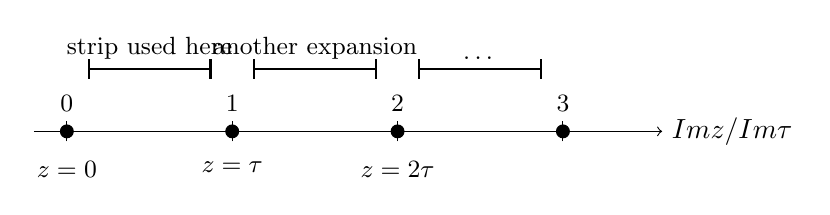
\begin{tikzpicture}[scale=1.05]
  \draw[->] (-0.4,0) -- (7.2,0) node[right] {$\operatorname{Im}z/\operatorname{Im}\tau$};
  \foreach \x/\l in {0/0, 2/1, 4/2, 6/3} \draw (\x,-0.12) -- (\x,0.12) node[above] {\small $\l$};
  \foreach \x in {0,2,4,6} \filldraw (\x,0) circle (2.2pt);
  \node[below] at (0,-0.25) {\small $z=0$};
  \node[below] at (2,-0.25) {\small $z=\tau$};
  \node[below] at (4,-0.25) {\small $z=2\tau$};
  \draw[thick,|-|] (0.25,0.75) -- (1.75,0.75) node[midway,above] {\small strip used here};
  \draw[thick,|-|] (2.25,0.75) -- (3.75,0.75) node[midway,above] {\small another expansion};
  \draw[thick,|-|] (4.25,0.75) -- (5.75,0.75) node[midway,above] {\small \dots};
\end{tikzpicture}
\caption{The poles of $A_{2,m}$ sit at $z\in\Z\tau+\Z$ (dots). Between two consecutive poles the
Fourier expansion of $A_{2,m}$ is a well-defined series, but it changes from one strip to the
next: that change is the wall crossing. All statements in this chapter use the first strip,
$|q|<|y|<1$.}\label{fig:dyons:strips}
\end{figure}

Two things are now checkable by pure arithmetic. First, that the multiple in
\eqref{eq:dyons:decomp} really is $p_{24}(m+1)$: the combination
$G_{m+1}-p_{24}(m+1)\,A\,A_{2,m}$ must vanish to second order at $y=1$, and it does, for
$m=1,2,3$; replacing $p_{24}(m+1)$ by $p_{24}(m+1)\pm1$ breaks it. Second --- and this is the
content, since the second-order condition follows from the symmetry $y\leftrightarrow y^{-1}$
--- the pole coefficient is $G_{m+1}(\tau,0)$, a constant in $\tau$, which is what makes the
subtraction $\tau$-independent at all.

\section{What is left: class numbers}\label{sec:dyons:classnumbers}

Fix $m=1$, the simplest magnetic charge. Removing the polar part leaves
$\Delta\psi^F_1=(G_2-324\,A\,A_{2,1})/A$, and the result is not a random-looking series. Recall
the Hurwitz--Kronecker class numbers\index{class number!Hurwitz--Kronecker}: for $N>0$, $H(N)$
counts $\SLZ$-classes of integral binary quadratic forms of discriminant $-N$, each weighted by
the reciprocal of the number of its automorphisms, with $H(0)=-1/12$ and $H(N)=0$ for $N<0$
\source{DMZ §7.1, ll.~2178--2192}. Concretely, count reduced forms $(a,b,c)$ with
$b^2-4ac=-N$, $|b|\le a\le c$ and $b\ge0$ when $|b|=a$ or $a=c$, weighting $a(x^2+y^2)$ by
$\tfrac12$ and $a(x^2+xy+y^2)$ by $\tfrac13$:
\begin{center}
\begin{tabular}{llll}
$N=3$: & $(1,1,1)$, weight $\tfrac13$ & $\Rightarrow$ & $H(3)=\tfrac13$\\
$N=4$: & $(1,0,1)$, weight $\tfrac12$ & $\Rightarrow$ & $H(4)=\tfrac12$\\
$N=7$: & $(1,1,2)$ & $\Rightarrow$ & $H(7)=1$\\
$N=12$: & $(1,0,3)$ and $(2,2,2)=2(1,1,1)$ & $\Rightarrow$ & $H(12)=1+\tfrac13=\tfrac43$\\
$N=15$: & $(1,1,4)$ and $(2,1,2)$ & $\Rightarrow$ & $H(15)=2$
\end{tabular}
\end{center}
(only $a$ with $3a^2\le N$ can occur, which is why the lists are short). The generating
function $\mathcal H(\tau,z)=\sum H(4n-r^2)q^ny^r$ \source{DMZ §7.2, ll.~2388--2392} is the
simplest mock Jacobi form there is.

\begin{theorem}[Immortal dyons at $m=1$; \TA\ through $q^3$, \TL\ for the interpretation]
\label{thm:dyons:m1}
$\displaystyle \Delta\psi^F_1=3E_4A-648\,\mathcal H$.
\end{theorem}

Two independent routes meet here. DMZ obtain the same statement by taking
$\phi=B^2/A$, computing its finite part, and \emph{recognizing} the numbers: the finite-part
coefficients $C(\Delta)$ and those of $E_4A$, called $C^*(\Delta)$, differ by exactly
$-288H(\Delta)$ \source{DMZ §8.5, ll.~3530--3558}. For instance at $\Delta=3$,
$152-248=-96=-288\cdot\tfrac13$, and at $\Delta=4$, $-636+492=-144=-288\cdot\tfrac12$. Our
route computes $\psi_1$ from the product \eqref{eq:dyons:dmvv}, subtracts $324A_{2,1}$ and
divides by $A$; the two answers agree coefficient by coefficient. With
$\phi^{\mathrm{opt}}_{2,1}=(B^2-E_4A^2)/(144A)$ \source{DMZ §9.2, ll.~3770--3776}, whose mock
part is $-2\mathcal H$, and $p_{24}(2)=324$, the arithmetic of
$\Delta\psi_1=\tfrac94 B^2/A+\tfrac34E_4A$ gives \cref{thm:dyons:m1} directly.

\subsection*{Worked example: the first coefficients of the immortal series}

It is worth seeing \cref{thm:dyons:m1} as numbers. Write
$\Delta\psi^F_1=\sum_{n,r}f(n,r)q^ny^r$. At order $q^0$ the form $A$ contributes
$y-2+y^{-1}$ and $\mathcal H$ contributes only $H(0)=-\tfrac1{12}$ at $r=0$, so
\begin{equation}\label{eq:dyons:immq0}
  f(0,\pm1)=3,\qquad f(0,0)=3\cdot(-2)-648\cdot\bigl(-\tfrac1{12}\bigr)=-6+54=48 .
\end{equation}
At order $q^1$ use the coefficients $C^*(\Delta)$ of $E_4A$ tabulated by DMZ
\source{DMZ §8.5, ll.~3546--3552}: $C^*(0)=-2$, $C^*(3)=248$, $C^*(4)=-492$. The discriminant
of $(n,r)=(1,0)$ is $\Delta=4$, of $(1,\pm1)$ is $3$, of $(1,\pm2)$ is $0$, so
\begin{align}\label{eq:dyons:immq1}
  f(1,0)&=3\cdot(-492)-648\cdot\tfrac12=-1800, &
  f(1,\pm1)&=3\cdot248-648\cdot\tfrac13=528,\notag\\
  f(1,\pm2)&=3\cdot(-2)+54=48 . &&
\end{align}
Every entry is an integer although $\mathcal H$ has denominators $12,3,2$: the combination
$3E_4A-648\mathcal H$ clears them, which is one reason the factor $648=54\cdot12$ appears. The
same integrality is what makes the Lean statement a comparison of integer lists.

For higher $m$ the pattern continues with a Hecke-like operator. $V_{k,t}$ acts on Fourier
coefficients by $C(\phi|V_{k,t};\Delta,r)=\sum_{d}d^{k-1}C(\phi;\Delta/d^2,r/d)$
\source{DMZ §4.4, ll.~1478--1490}, so for weight $2$, index $1$ and $t=p$ prime the effect on a
coefficient is $C(\Delta)\mapsto C(\Delta)+p\,C(\Delta/p^2)$ whenever $p^2\mid\Delta$. DMZ find
$\Phi^{\mathrm{opt}}_{2,p}=-\mathcal H|V_p$ for $p$ prime \source{DMZ §9.2, ll.~3846--3852},
with the explicit case splits
\begin{align}\label{eq:dyons:V2V3}
  C(\Phi^{\mathrm{opt}}_{2,2};\Delta)&=
  \begin{cases}-H(\Delta)&\Delta\equiv7\ (8),\\ -H(\Delta)-2H(\Delta/4)&4\mid\Delta,\end{cases}\notag\\
  C(\Phi^{\mathrm{opt}}_{2,3};\Delta)&=
  \begin{cases}-H(\Delta)&9\nmid\Delta,\\ -H(\Delta)-3H(\Delta/9)&9\mid\Delta.\end{cases}
\end{align}
Feeding these into \eqref{eq:dyons:516} with $p_{24}(3)=3200$, $p_{24}(4)=25650$ gives the
immortal counting functions at $m=2,3$:
\begin{align}\label{eq:dyons:m23}
  3\,\Delta\psi^F_2&=-9600\,\mathcal H|V_2+22E_4AB-10E_6A^2,\notag\\
  48\,\Delta\psi^F_3&=-1231200\,\mathcal H|V_3+467E_4AB^2-430E_6A^2B+203E_4^2A^3 .
\end{align}
Both are checked in \cref{sec:dyons:lean}, as is the failure of \eqref{eq:dyons:m23} when the
Hecke correction $2H(\Delta/4)$ is dropped --- the case split is not decoration.

\begin{physicsbox}[What the class numbers are counting]
A single-centred black hole of charge $(m,n,\ell)$ has a degeneracy that does not depend on
where one stands in moduli space. \Cref{thm:dyons:m1} says that for the smallest magnetic
charge those degeneracies, after removing a true Jacobi form, are class numbers: the number of
$\SLZ$-classes of binary quadratic forms of discriminant $-\Delta$, where $\Delta=4n-\ell^2$ is
the discriminant of the charge \eqref{eq:dyons:invariants}. The \TC\ reading that this is
``the black hole counting its own charge lattice'' is tempting and is not proved anywhere; the
identity of the two series is \TA\ through the order stated, and the physical meaning of
$\psi^F$ is \TL.
\end{physicsbox}

\section{Twining: are these integers characters?}\label{sec:dyons:twining}

\Cref{ch:moonshine} introduced the one test that separates moonshine from numerology:
replace dimensions by traces and ask whether the result is still a character. Apply it here.
For $g\in\Mtf$ with cycle shape (Frame shape) $\prod_k k^{e_k}$ on $24$ points
\source{CDH Table 14, ll.~4349--4364}, the twined analogue of \eqref{eq:dyons:goettsche} is
\begin{equation}\label{eq:dyons:twinedgoettsche}
  \sum_k T_k(g)\,p^k=\prod_{n\ge1}\frac{1}{\det(1-p^ng\,|\,\C^{24})}
  =\prod_{n\ge1}\prod_k(1-p^{nk})^{-e_k}.
\end{equation}
At $k=2$ this is the character of $V\oplus\mathrm{Sym}^2V$ with $V=\mathbf{1}\oplus\mathbf{23}$
the permutation representation. Since $\mathrm{Sym}^2\mathbf{23}=\mathbf{1}\oplus\mathbf{23}
\oplus\mathbf{252}$,
\begin{equation}\label{eq:dyons:hilb2}
  H^*(\mathrm{Hilb}^2\mathrm{K3})=3\cdot\mathbf{1}\oplus3\cdot\mathbf{23}\oplus\mathbf{252},
  \qquad 3+3\cdot23+252=324 ,
\end{equation}
a genuine character with non-negative multiplicities. The same holds through $k=4$. So the
$24$ of \cref{sec:dyons:product}, unlike the ``$27720$ lock'' of \cref{ch:dualscale}, passes
the twining test.

One can go further and twist the whole partition function. Cheng's twisted denominators
\source{Cheng §3.2, ll.~937--947} are
\begin{equation}\label{eq:dyons:twisted}
  \Phi_g(\Omega)=\ee^{4\pi\ii(\varrho,\Omega)}\prod_{\alpha}
  \exp\Bigl(-\sum_{k\ge1}\tfrac1k\,c_{g^k}(|\alpha|^2)\,\ee^{2\pi\ii k(\alpha,\Omega)}\Bigr),
\end{equation}
where $c_{g}$ are the Fourier coefficients of the twisted K3 elliptic genus $Z_g$ and $g^k$ is
read off the power maps of the character table \source{CDH Table 8, ll.~4172--4178}. The
twisted genera themselves come from the twining data of \cref{ch:moonshine}: with $\chi_g$ the
trace of $g$ on $\mathbf{1}\oplus\mathbf{23}$ \source{Cheng §2, ll.~455--460} and $F_g$ the
weight-$2$ forms of CDH,
\begin{equation}\label{eq:dyons:Zg}
  Z_g=\frac{\chi_g}{24}\,Z-F_g\,A ,
\end{equation}
which for the geometric classes $p=2,3,5,7$ is Cheng's (2.5) \source{Cheng §2, ll.~415--423}.
Expanding $\Phi_g^{-1}$ by Newton's identities gives twisted analogues $G^{(g)}_k$ of the
symmetric-product genera, and the outcome of the test is: every Fourier coefficient of
$G^{(g)}_1,G^{(g)}_2$, \emph{and} of the twisted immortal counting function at $m=1$, is a
virtual character of $\Mtf$ --- the multiplicities are integers, possibly negative. For
example the coefficient $-1800$ of $q^1y^0$ decomposes as
$2\cdot\mathbf{1}+2\cdot\mathbf{23}+2\cdot\mathbf{45}+2\cdot\overline{\mathbf{45}}
-\mathbf{231}-\overline{\mathbf{231}}+2\cdot\mathbf{252}-\mathbf{1035}'-\mathbf{1035}''$.

\begin{remark}[A printed sign]
Cheng states $c_g(-1)=-2$ when deriving the factorization of the pole
\source{Cheng §3.2, l.~960}. In the normalization used here --- and in Cheng's own (2.5) --- the
coefficient of $y^{\pm1}q^0$ in $Z_g$ is $+2$ for every class; the $q^0$ term is
$2y+(\chi_g-4)+2y^{-1}$. This is a sign convention, not a disagreement about the twisted
genera: the twisted products built with $+2$ reproduce the untwisted product at $g=1A$ and the
twined Göttsche numbers at $z=0$.
\end{remark}

\begin{pitfallbox}[This is $N=4$, not our universe]
Everything in this chapter lives in four-dimensional $N=4$ supergravity, where supersymmetry
protects the index and makes the count exact. Four-dimensional $N=4$ supersymmetry is not
chiral \source{Asp §7, ll.~2713--2716}, so the Standard Model is not among these vacua. The
results are statements about a mathematically controlled theory, \TL\ for their physical
reading and \TA\ only for the arithmetic; nothing here predicts anything measurable in our
world (\cref{ch:verdicts}).
\end{pitfallbox}

\section{What the machine has checked}\label{sec:dyons:lean}

The library \lean{DualScaleDyons} (six files) recomputes all of the above as exact integer
arithmetic on truncated series: a $q$-series is a list whose entries are Laurent polynomials in
$y$, stored as an offset plus a coefficient list, so no truncation in $y$ ever occurs. Every
theorem below depends only on \lean{propext}, \lean{Classical.choice} and \lean{Quot.sound};
the heavier ones are closed by \lean{decide +kernel}, which runs the decision procedure in the
kernel itself.

\begin{leanbox}[In Lean: the product, the guard, and Göttsche's numbers]
\begin{leancode}
theorem dmvv_reachable :
    [(5, 1), (4, 2), (2, 3)].all
      (fun kq : ℕ × ℕ => (dmvvDs kq.1 kq.2).all cAvailable) = true := by decide

theorem dmvv_unreachable_example :
    (dmvvDs 4 3).all cAvailable = false := by decide

theorem p24_values :
    (List.range 6).map p24 = [1, 24, 324, 3200, 25650, 176256] := by decide

theorem goettsche :
    (dmvv 5 1).map (fun Gk => Gk.map LP.eval1) =
      (List.range 6).map fun k => [p24 k, 0] := by decide +kernel
\end{leancode}
\textbf{Reading.} \lean{dmvv K Q} is the product \eqref{eq:dyons:dmvv} truncated at $p^K,q^Q$,
with exponents read from the \emph{computed} K3 elliptic genus. \lean{dmvv\_reachable} says
that for the three truncations used, every discriminant the product reads is available from
that genus; \lean{dmvv\_unreachable\_example} shows the guard is not vacuous. \lean{goettsche}
evaluates each $G_k$ at $y=1$ (\lean{LP.eval1} sums the coefficients) and finds
$[p_{24}(k),0]$: the value $p_{24}(k)$ at order $q^0$ and $0$ at order $q^1$, i.e.\ constancy
in $\tau$ as well as the value. \textbf{Proof idea.} Kernel evaluation of the finite product
and comparison of integer lists. \textbf{Not proved.} Convergence, modularity, or that $G_k$ is
the elliptic genus of a symmetric product (\TL, \source{DMZ §4.5, ll.~1688--1698}).
\end{leanbox}

\begin{leanbox}[In Lean: the additive formulas and the polar coefficient]
\begin{leancode}
theorem dmz_516_q2 :
    (List.range 5).all (fun k =>
      Ser.eqB (Ser.scale ((dmz516 2).getD k (1, [])).1 ((dmvv 4 2).getD k []))
        ((dmz516 2).getD k (1, [])).2) = true := by decide +kernel

theorem a2m_strip_eq_955 :
    [1, 2, 3].all (fun m => Ser.eqB (a2mRest m 6) (a2m955 m 6)) = true := by
  decide

theorem polar_part_removes_pole :
    [1, 2, 3].all (fun m => vanish2 (polarDefect m (p24 (m + 1)))) = true := by
  decide +kernel

theorem polar_coefficient_pinned :
    [1, 2, 3].all (fun m => !vanish2 (polarDefect m (p24 (m + 1) + 1)) &&
      !vanish2 (polarDefect m (p24 (m + 1) - 1))) = true := by decide +kernel
\end{leancode}
\textbf{Reading.} The first theorem is \eqref{eq:dyons:516} for $k\le4$ through order $q^2$,
with both sides multiplied by the printed denominators: the product route and the
$A,B,E_4,E_6$ route agree. The second says the direct expansion of \eqref{eq:dyons:A2m} in the
strip equals \eqref{eq:dyons:955}. The last two say $G_{m+1}-p_{24}(m+1)AA_{2,m}$ vanishes to
second order at $y=1$ and that $p_{24}(m+1)\pm1$ do not. \textbf{Caveat, as the file states.}
The second-order condition holds automatically by the $y\leftrightarrow y^{-1}$ symmetry, so
what these two discriminate is the first-order condition --- the pole coefficient. The full
second-order content at $m=1$ is \lean{immortal\_m1\_exact}, the exactness of the division by
$A$. \textbf{Tier} \TA\ for all four; \TL\ for ``$\psi^P$ counts two-centred states''.
\end{leanbox}

\begin{leanbox}[In Lean: immortal dyons are class numbers]
\begin{leancode}
theorem hurwitz_values :
    [0, 3, 4, 7, 8, 11, 12, 15].map h12 =
      [-1, 4, 6, 12, 12, 12, 16, 24] := by decide

theorem immortal_m1 :
    Ser.eqB immortalM1
      (Ser.sub (Ser.scale 3 (Ser.mul (e4 3) (phiA 3)))
        (Ser.scale 54 (hurwitzSer 3))) = true := by decide +kernel

theorem immortal_m1_needs_H :
    Ser.eqB immortalM1 (Ser.scale 3 (Ser.mul (e4 3) (phiA 3))) = false := by
  decide +kernel

theorem immortal_m2 :
    Ser.eqB (Ser.scale 3 (immortalM 2))
      (Ser.add (Ser.scale (-800) (hurwitzVSer 2 2 true))
        (Ser.add (Ser.scale 22 (mulAll [e4 2, phiA 2, phiB 2] 2))
          (Ser.scale (-10) (mulAll [e6 2, phiA 2, phiA 2] 2)))) = true := by
  decide +kernel
\end{leancode}
\textbf{Reading.} \lean{h12} computes $12H(N)$ by enumerating reduced forms, so
\lean{hurwitz\_values} is the hand computation of \cref{sec:dyons:classnumbers} checked by
machine ($12\cdot\tfrac13=4$, $12\cdot\tfrac12=6$, $12\cdot\tfrac43=16$).
\lean{immortalM1} is $(G_2-324AA_{2,1})/A$ computed from the product; \lean{immortal\_m1} is
\cref{thm:dyons:m1} with $648\mathcal H$ written as $54\cdot(12\mathcal H)$ to stay in $\Z$.
The control shows the class-number term is needed. \lean{immortal\_m2} is the first line of
\eqref{eq:dyons:m23}, with \lean{hurwitzVSer 2 2 true} the series $12(\mathcal H|V_2)$;
passing \lean{false} instead drops the Hecke correction and the identity fails
(\lean{immortal\_m2\_needs\_V2}). \textbf{Orders.} $q^3$ for $m=1$, $q^2$ for $m=2,3$.
\textbf{Tier} \TA\ for the identities; \TL\ for ``immortal'' and for mock modularity.
\end{leanbox}

\begin{leanbox}[In Lean: the twining test on the dyon sector]
\begin{leancode}
theorem frame_power_maps :
    powerMaps.all (fun pm => (List.range 26).all fun j =>
      fixedOfPower j pm.1 == fixedOfPower (pm.2.getD j 0) 1) = true := by decide

theorem twined_goettsche_k2 :
    (List.range 26).map (fun i => (twinedInner 2 i).1 / 244823040) =
      [3, 3, 0, 0, 0, 0, 1, 0, 0, 0, 0, 0, 0, 0, 0, 0, 0, 0, 0, 0, 0, 0, 0, 0,
       0, 0] := by decide +kernel

theorem twisted_dyons_are_characters :
    [1, 2].all (fun k => (List.range 3).all fun n =>
      (List.range 17).all fun i =>
      isVirtualChar (classFn (fun j => (dmvvTw j 2 2).getD k []) n
        ((i : ℤ) - 8))) = true := by decide +kernel

theorem c_minus_one :
    (List.range 26).all (fun j => cTw j (-1) == 2) = true := by decide +kernel
\end{leancode}
\textbf{Reading.} \lean{frame\_power\_maps} cross-checks two transcribed tables: the number of
points fixed by $g^p$, read from the Frame shape of $g$, equals the fixed-point count of the
class of $g^p$ given by the power maps, for all $26$ classes and $p=2,3,5,7,11,23$.
\lean{twined\_goettsche\_k2} is \eqref{eq:dyons:hilb2}: the multiplicities of $T_2$ on the $26$
irreducibles in this repository's ordering, $3,3,\dots,1$ at the entry $\mathbf{252}$.
\lean{twisted\_dyons\_are\_characters} says every Fourier coefficient of the twisted
$G^{(g)}_1,G^{(g)}_2$ through $q^2$ is a virtual character (all inner products with the
character table are integers and all irrational parts vanish). \lean{c\_minus\_one} is the sign
of the remark above. \textbf{Honest scope.} Given that the twisted genera are characters ---
which is Gannon's theorem, \TL\ --- the later steps are linear and class-independent, so
character-valuedness is expected; what is certified is the end-to-end computation from the
twining data of \cref{ch:moonshine} and the power maps.
\end{leanbox}

\begin{summarybox}
\begin{itemize}[leftmargin=*]
\item Quarter-BPS dyons on $\KT$ are counted by Fourier coefficients of $1/\Phi_{10}$; the
  three charges enter through the T-duality invariants $(m,n,\ell)=(M^2/2,N^2/2,N\cdot M)$.
\item $1/\Phi_{10}$ is built from one input, the K3 elliptic genus $Z=2\phi_{0,1}$, by the
  product \eqref{eq:dyons:dmvv}. At $z=0$ it collapses to $\prod(1-p^r)^{-24}$, so
  $G_k(\tau,0)=p_{24}(k)=1,24,324,3200,25650,176256$: Göttsche's numbers, the $24$ of K3
  propagated to all orders. The additive formulas \eqref{eq:dyons:516} are an independent check.
\item $\Delta\psi_m$ has a double pole at $z=0$ with coefficient $p_{24}(m+1)$. Subtracting the
  canonical polar part $p_{24}(m+1)A_{2,m}/\Delta$ leaves the finite part: two-centred
  (moduli-dependent, wall-crossing) versus single-centred (``immortal'') counts.
\item At $m=1$ the immortal counting function is $3E_4A-648\mathcal H$ with $\mathcal H$ the
  generating function of Hurwitz class numbers; at $m=2,3$ the same holds with
  $\mathcal H|V_2,\mathcal H|V_3$ and the case splits \eqref{eq:dyons:V2V3}.
\item Twining: the twined Göttsche numbers are characters of $\Mtf$
  ($H^*(\mathrm{Hilb}^2\mathrm{K3})=3\cdot\mathbf1\oplus3\cdot\mathbf{23}\oplus\mathbf{252}$),
  and every coefficient of the twisted partition functions, including the twisted immortal
  counts, is a virtual character.
\item Tiers: the arithmetic is \TA\ through the stated orders; ``counts black hole microstates'',
  mock modularity and the completion are \TL; $N=4$ in four dimensions is non-chiral, so none
  of this is a model of our universe.
\end{itemize}
\end{summarybox}

\section*{Exercises}
\addcontentsline{toc}{section}{Exercises}

\begin{exercise}[$\star$]\label{exo:dyons:p24}
Expand $\prod_{r\ge1}(1-p^r)^{-24}$ to order $p^3$ by hand and check $1,24,324,3200$. (Hint:
$(1-p)^{-24}$ alone gives $1,24,300,2600$; add the corrections from $r=2,3$.)
\end{exercise}

\begin{exercise}[$\star$]\label{exo:dyons:hurwitz}
Compute $H(8),H(11),H(16),H(19),H(20)$ by listing reduced forms, and check them against
$12H=12,12,18,12,24$.
\end{exercise}

\begin{exercise}[$\star$]\label{exo:dyons:limit}
Using \eqref{eq:dyons:ABq}, verify $A\sim(2\pi\ii z)^2$ and $B\to12$ as $z\to0$, and deduce
\eqref{eq:dyons:principal} from \eqref{eq:dyons:psiG}.
\end{exercise}

\begin{exercise}[$\star\star$]\label{exo:dyons:516}
Check the third relation of \eqref{eq:dyons:516} at order $q^0$: compute $B^2$ and $E_4A^2$ at
$q^0$ from \eqref{eq:dyons:ABq} and verify that $\tfrac94B^2+\tfrac34E_4A^2$ has the double
pole $324/(y-1)^2\cdot y$ expected from \eqref{eq:dyons:principal}.
\end{exercise}

\begin{exercise}[$\star\star$]\label{exo:dyons:strip}
Expand the $s=1$ term of \eqref{eq:dyons:A2m} for $m=1$ in the strip $|q|<|y|<1$, then again in
the strip $|q|^2<|y|<|q|$, and exhibit the first coefficient that differs. Explain which
physical statement the difference encodes.
\end{exercise}

\begin{exercise}[$\star\star$]\label{exo:dyons:sym2}
Prove $\mathrm{Sym}^2\mathbf{23}=\mathbf1\oplus\mathbf{23}\oplus\mathbf{252}$ for $\Mtf$ by
computing $\tfrac12(\chi_{23}(g)^2+\chi_{23}(g^2))$ on three classes of your choice and
comparing with the character table of \cref{ch:m24}; deduce \eqref{eq:dyons:hilb2}.
\end{exercise}

\begin{exercise}[$\star\star$]\label{exo:dyons:lean1}
In Lean, state and prove that the twined Göttsche numbers at $k=1$ reproduce the twisted Euler
characters: \lean{(List.range 26).map (fun j => twinedHilb j 1) = chiShadow}. (One line with
\lean{decide}; compare \lean{frame\_fixed\_points}.)
\end{exercise}

\begin{exercise}[$\star\star\star$]\label{exo:dyons:lean2}
Extend \lean{immortal\_m1} by one order in $q$: change the truncation from $3$ to $4$ in
\lean{immortalNum}, \lean{immortalM1} and \lean{hurwitzSer}, re-check that the division by $A$
is still exact, and measure the kernel time. Explain which step grows fastest and why the
reachability guard must be re-examined.
\end{exercise}

\begin{exercise}[$\star\star\star$]\label{exo:dyons:m3}
Derive the second identity of \eqref{eq:dyons:m23} from \eqref{eq:dyons:516},
$\phi^{\mathrm{opt}}_{2,3}=\psi^{\mathrm{opt}}_{0,4}/(12^4A)$ with
$\psi^{\mathrm{opt}}_{0,4}=B^4-6E_4A^2B^2+8E_6A^3B-3E_4^2A^4$, and $p_{24}(4)=25650$; check the
rational coefficients $467/48$, $-215/24$, $203/48$ before clearing denominators.
\end{exercise}

\section*{Further reading}
\addcontentsline{toc}{section}{Further reading}
\begin{itemize}[leftmargin=*]
\item Charges, invariants and the two counting problems: \source{DMZ §2.2--2.3, ll.~636--760};
  half-BPS degeneracies and $p_{24}$: \source{DMZ §3.4, ll.~1040--1071}; walls and contours:
  \source{DMZ §6, ll.~1900--2010}.
\item Jacobi forms of index $1$, the theta formulas and the coefficient table:
  \source{DMZ §4.3, ll.~1368--1430}; Hecke-like operators $U_s,V_{k,t}$:
  \source{DMZ §4.4, ll.~1470--1500}; the elliptic genus of K3 and the symmetric-product product
  formula: \source{DMZ §4.5, ll.~1660--1700}.
\item The Igusa form, its product representation and the additive formulas:
  \source{DMZ §5.1--5.2, ll.~1810--1900}; the polar/finite decomposition and its physics:
  \source{DMZ §1.1--1.2, ll.~196--240, 420--470}; class numbers and Example~5:
  \source{DMZ §7.1, ll.~2178--2196} and \source{DMZ §8.5, ll.~3530--3558}; optimal choices and
  $\mathcal H|V_p$: \source{DMZ §9.1--9.2, ll.~3600--3860}.
\item Twisted elliptic genera and twisted denominators: \source{Cheng §2, ll.~400--460} and
  \source{Cheng §3.2, ll.~900--990}; Frame shapes and power maps:
  \source{CDH Tables 8 and 14, ll.~4170--4209, 4349--4364}.
\item Within this book: the elliptic genus and $N=4$ characters, \cref{ch:ellgenus}; $\Mtf$ and
  its character table, \cref{ch:m24}; moonshine and the twining test, \cref{ch:moonshine};
  the computed moonshine data this chapter reuses, \cref{ch:moonshinecomputed}; what all of
  this does \emph{not} say about our universe, \cref{ch:verdicts}.
\end{itemize}
